% Preamble
\documentclass[12pt, a4paper]{article}
\title{\emph{Arch Linux} \\\emph{Installation Guide}}
\author{Written by Volunteers}
\date{May 17, 2021}

% Packages
\usepackage{xcolor}
\usepackage{hyperref}
\usepackage{graphicx}
\graphicspath{{images/}}
% Body
\begin{document}
\maketitle

\section*{Important Notes :}
\paragraph{}
This installation guide is \emph{specialized} for computers with \href{https://en.wikipedia.org/wiki/BIOS}{\textcolor{blue}{\emph{BIOS}}} firmware.
\paragraph{}
This guide is based on the \emph{ArchWiki installation} \href{https://wiki.archlinux.org/index.php/Installation_guide}{\emph{\textcolor{blue}{guide}}}.

\paragraph{}
After reading this guide you should consider reading this one :
\begin{LARGE}
	\paragraph{}
	\centering
	\emph{"Things to do After Installing Arch"}\\
\end{LARGE}

\begin{center}
	
\includegraphics[scale=0.4]{cc-zero}
\end{center}

\newpage
\begin{enumerate}
	\item Download the iso image
	\item Verify \emph{signature}
	\item Prepare an \emph{installation medium}
	\item Connect to the internet
	\item Partition the disks
	\item Format the partitions
	\item Mount the file systems
	\item Install essential packages
	\item Fstab
	\item Chroot
	\item Localization
	\item Network configuration
	\item Root password
	\item Boot loader
	\item Reboot
	\item Set time zone
	\item Select the mirror
	\item Install \emph{Desktop Environment}
	\item Post-installation
\end{enumerate}

\newpage
\section{Download the iso image}
\paragraph{} 
You can  \href{https://archlinux.org/download/}{\textcolor{blue}{\emph{download}}} Arch Linux from its official website.

\section{Verify signature}
\paragraph{}
 Install GnuPG on your Linux distribution and \href{https://wiki.archlinux.org/index.php/Installation_guide#Verify_signature}{\textcolor{blue}{\emph{verify}}} the iso \emph{signature}.

\section{prepare an installation medium}
\paragraph{}
First of all plug in your usb flash drive to your device usb port.

\begin{center}
	\$ lsblk -f
\end{center}

 \paragraph{}
With this command you can find your usb flash drive name.\\\\
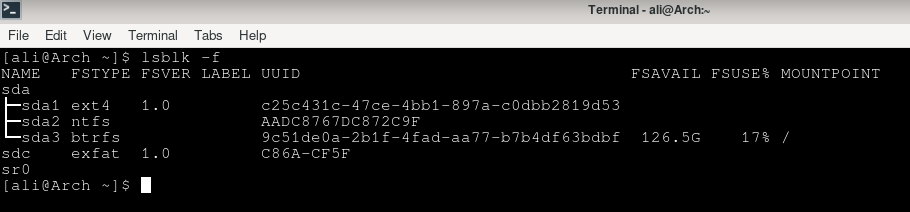
\includegraphics[scale=0.5]{lsblk.png}

\paragraph{}
Now you can make a \emph{bootable} usb flash drive with \emph{"dd"} utility.

\begin{center}
	\# dd bs=4M status=progress if=arch.iso  of=/dev/sdc oflag=sync
\end{center}

\begin{enumerate}
	\item Enter the iso image path instead of \emph{"arch.iso"}
	\item Enter your usb flash drive name instead of \emph{"/dev/sdc"}
\end{enumerate}

\section{Connect to the internet}
\paragraph{}
I recommend you to use Ethernet instead of Wifi.

\section{Partition the disks}
\paragraph{}
I want to make a \emph{swap file} instead of \emph{swap partition}. So i make one partiton.

\paragraph{}
Enter this command :
\begin{center}
	\# cfdisk /dev/sda
\end{center}

\begin{enumerate}
	\item Make one partition and select \emph{"Linux (83)"} as its type
	\item Set the \emph{"bootable flag"} for this partition
	\item Write partition table to disk and select \emph{"Quit"}
\end{enumerate}

\section{Format the partitions}
\paragraph{}
I prefer the Btrfs format :
\begin{center}
	\# mkfs.btrfs /dev/sda1
\end{center}

\section{Mount the file system}
\paragraph{}
Mount your [root] partition to "/mnt" :

\begin{center}
	\# mount /dev/sda1 /mnt
\end{center}

\section{Install essential packages :}
\paragraph{}
Use pacstrap to install essential packages.

\begin{center}
	\# pacstrap /mnt base linux linux-firmware man-db man-pages vim
\end{center}
 
 \section{Fstab}
 \paragraph{}
 Generate an \href{https://wiki.archlinux.org/index.php/Fstab}{\textcolor{blue}{\emph{fstab}}} file with \emph{"gen-fstab"} command :
 
 \begin{center}
 	\# genfstab -U /mnt $>>$ /mnt/etc/fstab
 \end{center}
 
 \section{Chroot}
 \paragraph{}
 Change root into the new system :
 
 \begin{center}
 	\# arch-chroot /mnt
 \end{center}

\section{Localization}
\paragraph{}
For this part folow this instruction :

\begin{center}
	\begin{tabular}{|c|} \hline
		\# vim /etc/locale.gen\\ \hline
		\textit{Uncomment} the \emph{"en\_US.UTF-8 UTF-8"}\\ \hline
		\textit{Uncomment} other \emph{locales} , if needed\\ \hline
		\# locale-gen\\ \hline
		\# vim /etc/locale.conf\\ \hline
		\emph{Add} \emph{"LANG=en\_US.UTF-8"} and save changes\\ \hline
	\end{tabular}
\end{center}

\section{Network configuration}
Folow this instruction :

\begin{enumerate}
	\item \# vim /etc/hostname
	\item \textit{Enter} your \emph{"hostname"} and save the changes
	\item Add matching entries to \emph{"/etc/hosts"} :

\begin{center}
	\begin{tabular}{|ll|} \hline
		127.0.0.1 &  localhost\\ \hline
		::1				 &  localhost\\ \hline
		127.0.1.1 &  myhostname.localdomain	\space{myhostname}\\ \hline
	\end{tabular}
\end{center}

	\item Replace \emph{"myhostname"} with your hostname
	\item Replace \emph{"localdomain"} with your localdomain
	\item Install and start network manager :
	
	\begin{center}
		\begin{tabular}{|c|} \hline
			\# pacman -S networkmanager\\ \hline
			\# systemctl enable NetworkManager\\ \hline
		\end{tabular}
	\end{center}
	
	\item Now you can use \emph{"nmcli"} \& \emph{"nmtui"} utilities to connect to the internet
\end{enumerate}

\section{Root password}
\paragraph{}
Set the root password with this command :
\begin{flushleft}
	\# passwd
\end{flushleft}
\paragraph{}
Now enter the \emph{"New password"}. And \emph{again} !

\section{Boot loader}
\paragraph{}
Choose and install a Linux-capable \textit{boot loader} and install microcode.
\begin{enumerate}
	\item \# pacman -S grub (boot loader)
	\item Install microcode :
	
		\begin{center}
		\begin{tabular}{|c|} \hline
			\# pacman -S intel-ucode (for intel processors)\\ \hline
			\# pacman -S amd-ucode (for amd processors)\\ \hline
		\end{tabular}
	\end{center}
	
	\item Install \emph{"os-prober"} \& \emph{"ntfs-3g"} :
	
			\begin{center}
		\begin{tabular}{|c|} \hline
			\# pacman -S os-prober ntfs-3g\\ \hline
			\# grub-install $--$target=i386-pc /dev/sda\\ \hline
			\# grub-mkconfig -o /boot/grub/grub.cfg\\ \hline
		\end{tabular}
	\end{center}
\end{enumerate}

\section{Reboot}
\paragraph{}
Exit the chroot environment by typing \emph{"exit"} or pressing \emph{"Ctrl+d"}. 
\paragraph{}
Finally, restart the machine by typing \emph{"reboot"}.

\section{Set time zone}
\paragraph{}
Follow this instruction :

\begin{enumerate}
	\item \# timedatectl set-ntp true

\begin{center}
	\begin{tabular}{|c|} \hline
		\# ln -sf /usr/share/zoneinfo/Region/City /etc/localtime\\ \hline
	\end{tabular}
\end{center}
	
	\item Replace \emph{"/Region/City"} with your region and city. this one is for Iran 
	
	\begin{center}
		\begin{tabular}{|c|} \hline
			\# ln -sf /usr/share/zoneinfo/Asia/Tehran /etc/localtime\\ \hline
		\end{tabular}
	\end{center}
	
	\item \# hwclock $--$systohc
\end{enumerate}

\section{Select the mirror}
\paragraph{}
You can find the fastest mirror by this command :

\begin{center}
	\resizebox{\textwidth}{!}{%
	\begin{tabular}{|c|} \hline
		\# pacman -S reflector\\ \hline
		\# reflector $--$country Germany $--$age 12 $--$protocol https $--$sort rate $--$save /etc/pacman.d/mirrorlist\\ \hline
		\# pacman -Syy \\\hline
	\end{tabular}
}
\end{center}

\paragraph{}
You can replace \emph{"Germany"} with other countries.

\section{Install \emph{Desktop Environment}}
I show you how to install \emph{xfce4} with \emph{lightdm} :
\begin{enumerate}
	\item Install graphics card driver :
	\begin{center}
		\begin{tabular}{|c|} \hline
			\# pacman -S xf86-video-amdgpu xf86-video-ati\\ \hline
		\end{tabular}
	\end{center}

	\item For other graphics cards search \emph{"xf86-video"} and find the driver name
\begin{center}
	\begin{tabular}{|c|} \hline
		\# pacman -Ss xf86-video\\ \hline
		\# pacman -S xf86-video-nouveau (for Nvidia graphic cards)\\ \hline
	\end{tabular}
\end{center}

	\item Install lightdm \& xfce4
\begin{center}
	\begin{tabular}{|c|} \hline
		\# pacman -S xorg-server\\ \hline
		\# pacman -S lightdm lightdm-gtk-greeter lightdm-gtk-greeter-settings\\ \hline
		\# systemctl enable lightdm\\ \hline
		\# pacman -S xfce4\\ \hline
		\# reboot\\ \hline
	\end{tabular}
\end{center}
\end{enumerate}

\newpage
\section{Post-installation}
\paragraph{}
For this part you can read my another guide about Arch Linux :

\begin{Large}
	\paragraph{}
	\centering
	\emph{"Things to do After Installing Arch"}
\end{Large}

\begin{enumerate}
	\item Login as \emph{root} and create a user  and add it to the \emph{"wheel"} group :
	
	\begin{center}
		\begin{tabular}{|c|} \hline
			\# pacman -S sudo\\ \hline
			\# useradd -mG wheel [user name]\\ \hline
			\# vim  /etc/sudoers\\ \hline
			Edit the sudoers file like this :\\
			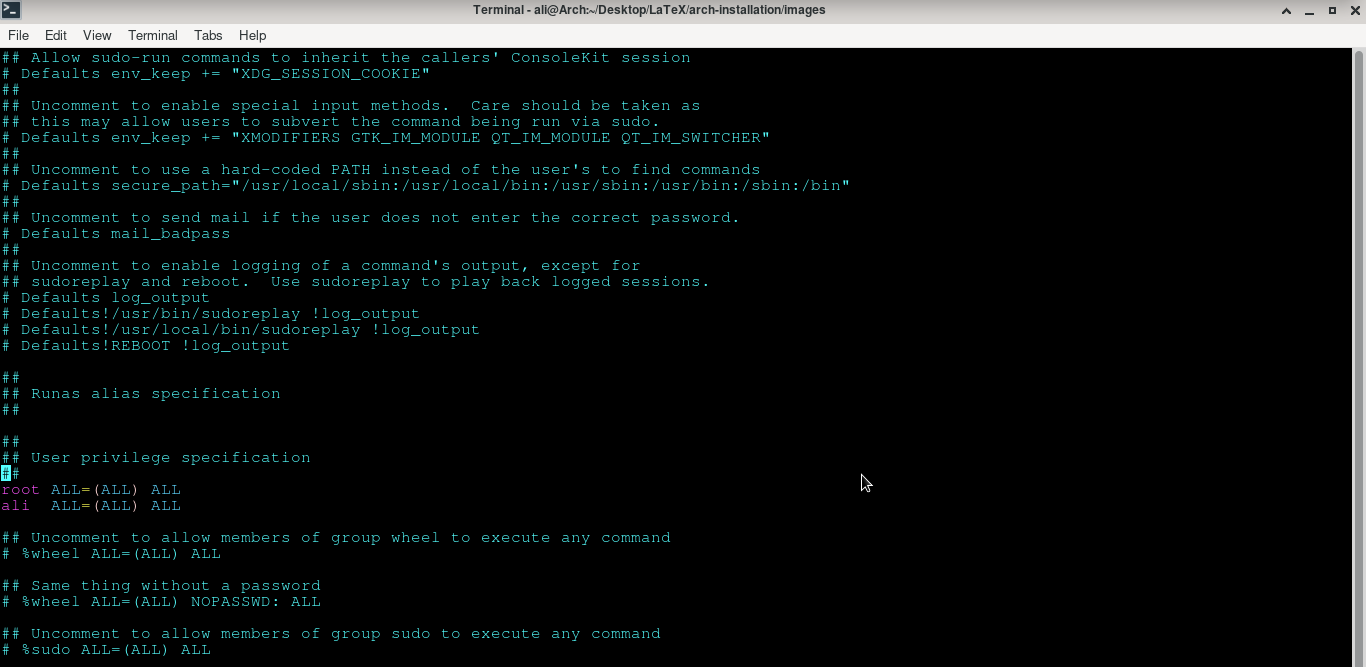
\includegraphics[scale=0.3]{sudoers.png}\\
			replace \emph{"ali"} with your \emph{"user name"}\\ \hline
		\end{tabular}
	\end{center}
	
	\item Now you can use \emph{"sudo"} for your commands 
	\item you can make swapfile (4G) by this instruction :
	
		\begin{center}
		\begin{tabular}{|c|} \hline
			\# mkdir /swap\\ \hline
			\# chattr +C /swap (for Btrfs)\\ \hline
			\# cd /swap\\ \hline
			\# dd if=/dev/zero of=/swap/swapfile bs=1024 count=4M\\ \hline
			\# chmod 600 /swap/swapfile\\ \hline
			\# mkswap /swap/swapfile\\ \hline
			\# swapon /swap/swapfile\\ \hline
		\end{tabular}
	\end{center}
	
	\item you can set any size for swapfile (size = bs$\times$count)
	\item edit fstab file :
	
	\begin{center}
		\begin{tabular}{|c|} \hline
			\# vim /etc/fstab\\ \hline
			Add these lines to the fstab file :\\
			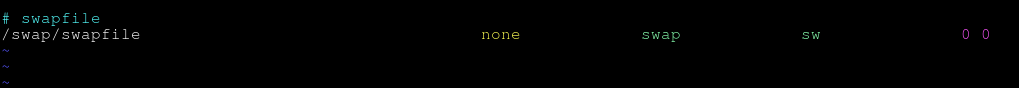
\includegraphics[scale=0.4]{swapfile.png}\\ \hline
			Save changes !\\ \hline
			\# reboot\\ \hline
		\end{tabular}
	\end{center}
	
	\paragraph{}
	Arch Wiki provides a \href{https://wiki.archlinux.org/index.php/General_recommendations}{\emph{\textcolor{blue}{general recommendations}}} for this purpose.
	
	\begin{Huge}
		\begin{center}
			\textit{END !}
		\end{center}
	\end{Huge}
 
\end{enumerate}
\end{document}
